\documentclass[conference]{IEEEtran}
\IEEEoverridecommandlockouts
\usepackage{cite}
\usepackage{amsmath,amssymb,amsfonts}
\usepackage{graphicx}
\usepackage{booktabs}
\usepackage{multirow}
\usepackage{tabularx}
\usepackage{url}
\usepackage{microtype}

% --- Custom Command to split authors across balanced centered rows in IEEEtran ---
\makeatletter
\newcommand{\linebreakand}{%
  \end{@IEEEauthorhalign}
  \hfill\mbox{}\par
  \mbox{}\hfill\begin{@IEEEauthorhalign}
}
\makeatother

\def\BibTeX{{\rm B\kern-.05em{\sc i\kern-.025em b}\kern-.08em
    T\kern-.1667em\lower.7ex\hbox{E}\kern-.125emX}}

\begin{document}

\title{TokenShield: A Real-Time, Behavioral-Based Multi-Signal Engine for Detecting and Automatically Mitigating Session Hijacking}

\author{%
% --- ROW 1: 2 Authors ---
\IEEEauthorblockN{1\textsuperscript{st} Arvind R. Bhagat Patil}
\IEEEauthorblockA{\textit{Dept. of Computer} \\
\textit{Technology}\\
\textit{Yeshwantrao Chavan}\\
\textit{College of Engineering}\\
Nagpur, India \\
arbhagatpatil@gmail.com}
\and
\IEEEauthorblockN{2\textsuperscript{nd} Aman Kshirsagar}
\IEEEauthorblockA{\textit{Dept. of Artificial Intelligence} \\
\textit{and Data Science}\\
\textit{Yeshwantrao Chavan}\\
\textit{College of Engineering}\\
Nagpur, India \\
amankshirsagar@gmail.com}
\linebreakand
% --- ROW 2: 3 Authors ---
\IEEEauthorblockN{3\textsuperscript{rd} Vedant Dhamele}
\IEEEauthorblockA{\textit{Dept. of Artificial Intelligence} \\
\textit{and Data Science}\\
\textit{Yeshwantrao Chavan}\\
\textit{College of Engineering}\\
Nagpur, India \\
vedantdhamele@gmail.com}
\and
\IEEEauthorblockN{4\textsuperscript{th} Yash Shashank Pachhade}
\IEEEauthorblockA{\textit{Dept. of Artificial Intelligence} \\
\textit{and Data Science}\\
\textit{Yeshwantrao Chavan}\\
\textit{College of Engineering}\\
Nagpur, India \\
yashp2906@gmail.com}
\and
\IEEEauthorblockN{5\textsuperscript{th} Yash Nandanwar}
\IEEEauthorblockA{\textit{Dept. of Artificial Intelligence} \\
\textit{and Data Science}\\
\textit{Yeshwantrao Chavan}\\
\textit{College of Engineering}\\
Nagpur, India \\
yashnandanwar2005@gmail.com}
}

\maketitle

\vspace{10pt}
\begin{abstract}
Session hijacking involves the theft and replay of valid authentication tokens to impersonate legitimate users. Because bearer tokens remain cryptographically valid until expiration, perimeter firewalls, fixed-window rate throttling, and login-bound multi-factor authentication cannot protect active sessions once a token is compromised. This paper presents TokenShield, a framework-agnostic security middleware designed for continuous, request-level session protection. The engine evaluates eight cross-modal telemetry signals per HTTP request: IP reputation, request velocity, session consistency, payload anomalies, non-PII behavioral biometrics, geographical velocity, endpoint sensitivity, and request sequence transitions. TokenShield incorporates an LSTM sequence autoencoder that models temporal workflow trajectories across a rolling 10-request window to detect out-of-order API exploitation. Upon crossing risk thresholds, the system executes an autonomous eight-stage mitigation cascade encompassing cache token invalidation, reverse-proxy edge blocking, device fingerprint blacklisting, and step-up authentication. To preserve user privacy, the architecture stores only running statistical summaries rather than raw input logs. Evaluated on a held-out benchmark of 143,781 samples drawn from 12 empirical dataset pipelines, the meta-classifier achieves an ROC-AUC of 0.8943 and 96.90\% recall at a 0.50 triage threshold (40.03\% FPR, 72.52\% precision), while its calibrated autonomous mitigation threshold ($\tau \ge 0.85$) operates at 1.05\% FPR with 98.18\% precision and an average inference latency of 11.25 ms on Apple M2 hardware. Because public datasets lack authentic session hijacking labels, these evaluations constitute an empirical proxy benchmark.
\end{abstract}

\begin{IEEEkeywords}
anomaly detection, automated incident response, behavioral biometrics, continuous authentication, intrusion detection, session hijacking, token theft, web security
\end{IEEEkeywords}

\section{Introduction}
Stateless, token-based authentication services---principally JSON Web Tokens (JWT)~\cite{ref1}---provide horizontal scalability for distributed web applications. However, bearer credential architectures inherently couple authorization to the token itself rather than the physical user. When an adversary acquires an active token via cross-site scripting (XSS), malicious extensions, local storage extraction, or network interception, the backend lacks cryptographic mechanisms to differentiate legitimate owners from impersonators. With a valid stolen token, adversaries can authorize illicit wire transfers in financial portals, exfiltrate Protected Health Information (PHI) from clinical systems, or compromise administrative interfaces in SaaS platforms before token expiry~\cite{ref2}.

Conventional perimeter defenses fail to protect this post-authentication attack surface. Web Application Firewalls (WAFs) filter on known exploit signatures (e.g., SQLi, XSS) and remain blind to syntactically valid HTTP requests bearing legitimate tokens. Fixed-window IP rate limiting is routinely bypassed using low-and-slow replay schedules or rotating residential proxies. Furthermore, Multi-Factor Authentication (MFA) and FIDO2 passkeys authenticate credentials only at the login boundary, offering no continuous verification throughout session lifecycles.

To mitigate this systemic vulnerability, this paper introduces TokenShield, a continuous request-level risk evaluation and automated mitigation engine. Rather than treating authentication as an isolated login event, TokenShield inspects every authenticated HTTP request as an autonomous trust decision. The system continuously evaluates client telemetry to verify session continuity and dynamically executes defensive countermeasures. TokenShield was implemented and evaluated against NeoVault, a production-grade digital banking demonstrator. However, its detection engine is strictly framework-agnostic, ingesting ubiquitous telemetry signals including IP reputation, geographical velocity, device configuration entropy, non-PII behavioral biometrics, endpoint risk, and sequential request trajectories.

This paper provides the following primary contributions:
\begin{itemize}
    \item \textbf{An 8-Signal Multi-Tiered Anomaly Detection Architecture:} We formulate a composite scoring model that integrates network telemetry, geographical plausibility, device entropy, streaming non-PII behavioral biometrics (keystroke hold/flight times and cursor velocity using Welford's algorithm), and sequential request modeling via an LSTM autoencoder over a 10-request rolling window.
    \item \textbf{Empirical Multi-Source Benchmark Corpus:} We consolidate an empirical evaluation corpus of 958,534 real-world records spanning network telemetry (UNSW-NB15~\cite{ref5}, CIC-IoT 2023~\cite{ref13}, NSL-KDD, Bot-IoT), behavioral biometrics (CMU Keystroke~\cite{ref11}, Balabit Mouse Dynamics, KeyRecs), and temporal web request logs (NASA HTTP, CSIC 2010, Wikipedia Clickstream) across 12 processing pipelines and 23 sub-corpora.
    \item \textbf{Rigorous Empirical Evaluation:} On a strict held-out test split of 143,781 samples, the meta-classifier achieves an ROC-AUC of 0.8943. At its triage threshold ($\tau = 0.50$), it delivers 96.90\% recall (72.52\% precision, 40.03\% FPR); at its high-confidence autonomous mitigation threshold ($\tau \ge 0.85$), it operates at 1.05\% FPR with 98.18\% precision. The complete feature extraction and inference pipeline sustains an average latency of 11.25 ms (P95: 14.97 ms) on Apple M2 hardware.
    \item \textbf{Autonomous Multi-Stage Mitigation Engine:} When anomaly scores exceed calibrated thresholds, TokenShield triggers an autonomous multi-layer response without manual intervention. This pipeline executes cache token revocation, edge-proxy IP filtering, firewall rule synchronization, device-fingerprint blacklisting, account-level lockouts, subnet (/24) throttling, Security Operations Center (SOC) alert dispatch, and Server-Sent Event (SSE) dashboard updates.
    \item \textbf{Decoupled Middleware Architecture:} We deliver the system as a standalone REST microservice accompanied by a drop-in SDK, allowing arbitrary web and mobile architectures to enforce zero-trust continuous authentication out of the box.
\end{itemize}

\section{Related Work}

\subsection{Anomaly-Based Intrusion Detection and Benchmarks}
Anomaly-based intrusion detection operates on the premise that malicious activity resides in sparse, outlier regions of a learned feature space. Liu et al.\ formalized this through the Isolation Forest algorithm, isolating anomalous instances via recursive random partitioning with linear time complexity suitable for low-latency streaming~\cite{ref3}. To benchmark detection algorithms, Sharafaldin et al.\ developed the CIC-IDS2017/2018 benchmark corpus containing benign traffic alongside denial-of-service, brute-force, web exploits, and infiltration attacks~\cite{ref4}. Similarly, Moustafa and Slay established the UNSW-NB15 dataset using the IXIA testbed to combine contemporary attack vectors with realistic background network flows~\cite{ref5}.

\subsection{Client Authentication and Device Fingerprinting}
In identity verification, Freeman et al.\ modeled login legitimacy probabilistically using IP reputation, device signatures, and geographical velocity~\cite{ref6}. Investigating client uniqueness, Eckersley demonstrated that configuration entropy gathered from browser headers and canvas attributes provides sufficient distinctiveness to track devices without persistent identifiers~\cite{ref7}. Nikiforakis et al.\ expanded on this foundation by surveying cookieless fingerprinting techniques that exploit client JavaScript APIs and environment attributes to detect session tampering~\cite{ref8}. Complementary industrial protocols have emerged to bind credentials cryptographically, including OAuth 2.0 Demonstrating Proof-of-Possession (DPoP, RFC 9449)~\cite{ref14} and mutual-TLS client certificate-bound tokens (RFC 8705). However, cryptographic token binding requires client-side hardware keystore support and widespread infrastructure modification, leaving bearer tokens dominant in consumer web applications.

\subsection{Behavioral Biometrics}
Behavioral biometrics offers continuous identity verification without specialized hardware. Killourhy and Maxion established foundational benchmarks for keystroke dynamics, demonstrating that individual typing rhythms (hold times and inter-key latencies) serve as continuous authentication vectors~\cite{ref9,ref11}. Acien et al.\ scaled this concept using TypeNet, a deep recurrent neural network that models temporal typing dynamics over extended typing sequences~\cite{ref10}. Broader surveys by Shadman et al.\ confirm that multi-modal fusion of typing and cursor dynamics significantly reduces equal error rates compared to single-modality channels~\cite{ref12}. Despite these developments, broken authentication and session hijacking remain ranked among the top web application vulnerabilities by OWASP~\cite{ref2,ref15}.

\subsection{Limitations of Surveyed Literature}
The surveyed literature exhibits three structural limitations (cf.\ Table~\ref{tab:comparison}):
\begin{itemize}
    \item \textbf{Single-modal silos:} Prior defenses examine telemetry dimensions in isolation. None unify heterogeneous network, client, biometric, and payload signals into a composite risk score.
    \item \textbf{Stateless point-in-time evaluation:} Existing anomaly engines treat each HTTP request independently, failing to detect out-of-order execution, token replay, or abrupt workflow leaps.
    \item \textbf{Open-loop architectures:} Prior works decouple detection from mitigation. Scoring is written to log files for retrospective investigation rather than triggering closed-loop automated enforcement.
\end{itemize}

\section{TokenShield System Architecture}

TokenShield operates as a modular, framework-agnostic middleware layer interposed between external ingress traffic and internal application services (Fig.~\ref{fig:arch}). The runtime architecture spans five functional layers:
\begin{enumerate}
    \item \textbf{Ingress and Perimeter Enforcement:} Inbound HTTP requests terminate at an Nginx edge reverse proxy enforcing perimeter TLS termination and rate limits.
    \item \textbf{Telemetry Ingestion and Context Extraction:} Application-level middleware intercepts all incoming HTTP requests prior to controller dispatch via a global \texttt{before\_request} hook.
    \item \textbf{Multi-Tier Anomaly Scoring Engine:} Extracted telemetry is transformed into normalized risk vectors evaluated against unsupervised and ensemble classifiers.
    \item \textbf{State Management and Distributed Cache:} Volatile session state, running statistical summaries, and dynamic blacklists are managed in-memory via Redis.
    \item \textbf{Automated Cascading Mitigation Pipeline:} When anomaly scores exceed operational thresholds, mitigation routines execute progressive countermeasures.
\end{enumerate}

\begin{figure}[!htbp]
\centering
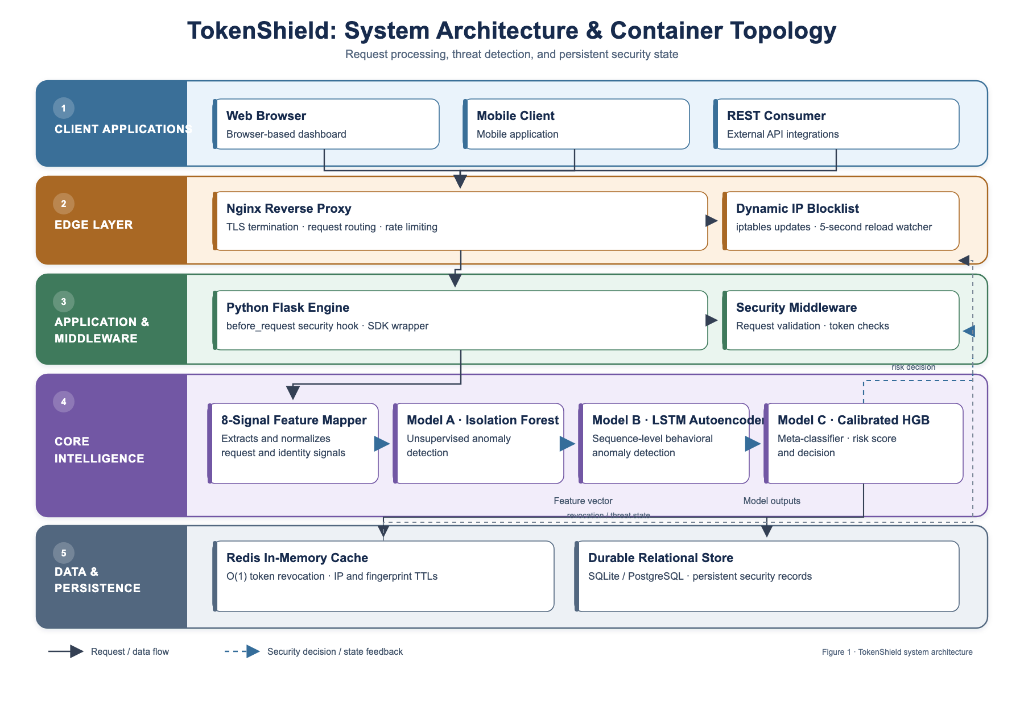
\includegraphics[width=\columnwidth,keepaspectratio]{fig1_system_architecture.png}
\caption{TokenShield multi-tier system architecture: Telemetry ingestion, distributed caching, machine learning inference, and automated mitigation.}
\label{fig:arch}
\end{figure}

\begin{table}[!htbp]
\caption{System Modules: Technique and Primary Benefit}
\label{tab:modules}
\centering
\resizebox{\columnwidth}{!}{%
\renewcommand{\arraystretch}{1.3}
\begin{tabular}{|l|p{4.2cm}|p{4.6cm}|}
\hline
\textbf{Module} & \textbf{Technique / Algorithm} & \textbf{Primary Security Benefit} \\ \hline\hline
\textbf{Edge Ingestion} & Dynamic Nginx Reverse Proxy + Blocklist Watcher & Enforces sub-5s perimeter packet dropping before engine compute. \\ \hline
\textbf{Network Telemetry} & CIDR Subnet Trie + Sliding-Window Rate Counter (Redis) & Flags distributed brute force, Tor routing, and IP drift instantly. \\ \hline
\textbf{Behavioral Biometrics} & Non-PII Keystroke / Mouse Dynamics + Welford's Algorithm & Detects credential-replay attacks and automated headless bots. \\ \hline
\textbf{Sequence Autoencoder} & Deep LSTM Autoencoder over 10-Request Sliding Window & Catches workflow skipping and direct API privilege jumping. \\ \hline
\textbf{Model A (First-Pass)} & 300-Tree Isolation Forest (Calibrated Cutoff: $0.4334$) & Fast sub-3ms isolation of novel anomalies with FPR $\le 5\%$. \\ \hline
\textbf{Model C (Meta-Classifier)} & HistGradientBoosting + Platt Sigmoid Calibration & High-confidence lockdown (\textbf{98.18\% precision}, \textbf{1.05\% FPR}). \\ \hline
\textbf{Autonomous Mitigation} & 8-Stage Progressive Cascading Pipeline & Instant token revocation, edge blocking, and account locking. \\ \hline
\end{tabular}%
}
\end{table}

\subsection{State Partitioning and Data Persistence}
To sustain sub-15 ms average processing latencies along the critical path, state management is partitioned between volatile in-memory storage and durable relational persistence. The Redis in-memory cache provides $\mathcal{O}(1)$ lookups for revoked token blacklists (\texttt{ts:block:*}), IP velocity counters (\texttt{ts:vel:*}), banned device fingerprints (\texttt{ts:fp:*}), and geographic coordinates (\texttt{ts:geo:*}), with in-process dictionary fallbacks in the event of Redis downtime. The relational persistence layer uses SQLAlchemy to persist user accounts, audited session lifecycles, and security incident forensics onto an ACID-compliant relational database.

\begin{figure}[!htbp]
\centering
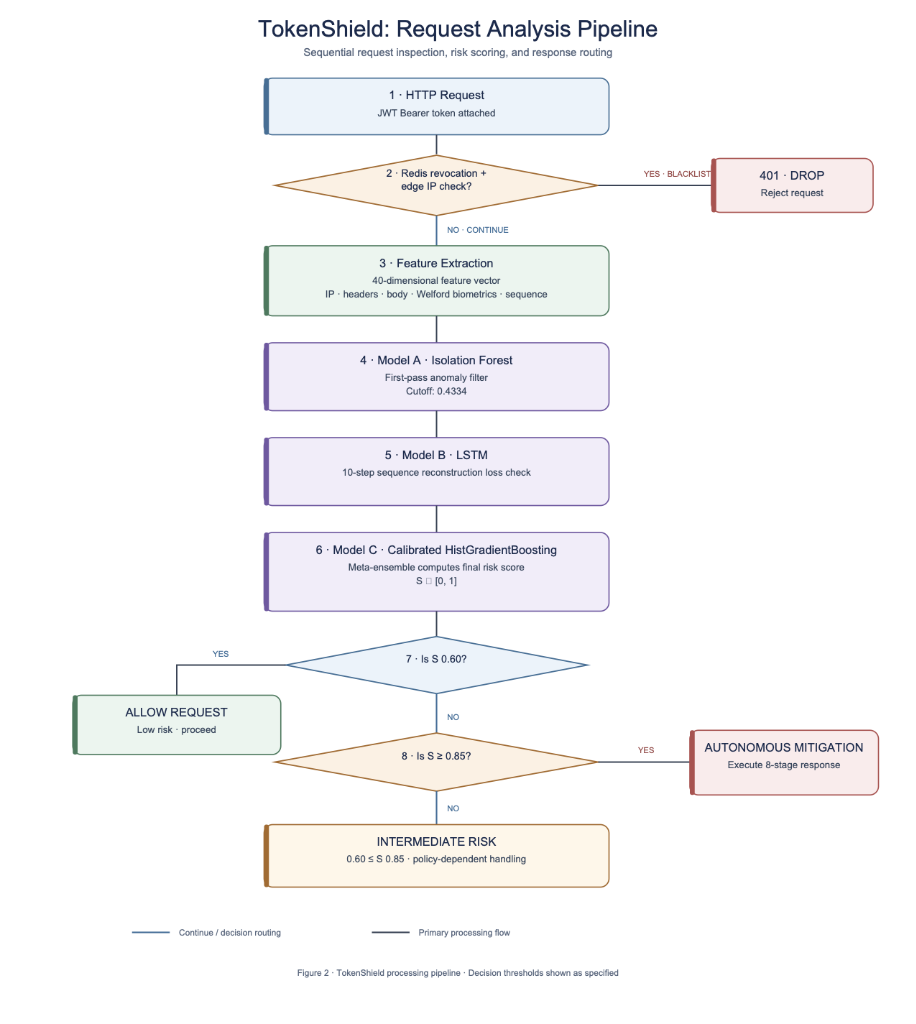
\includegraphics[width=\columnwidth,keepaspectratio]{fig2_request_pipeline.png}
\caption{TokenShield processing pipeline: Sequential request inspection, risk scoring, and response routing.}
\label{fig:pipeline}
\end{figure}

\section{Core Threat Detection and Risk Scoring Formulation}

Every authenticated request is mapped to an 8-dimensional signal vector $\mathbf{s} = [s_1, s_2, \dots, s_8]^T$, where each component represents a normalized risk metric bounded in $[0, 1]$:

\subsubsection{Signal 1: IP Reputation and Threat Intelligence ($s_1$)}
Evaluates the originating IP against known malicious infrastructure:
\begin{equation}
s_1 = \max \left( I_{\text{Tor}}, I_{\text{VPN}}, I_{\text{Abuse}} \right) \in [0.0, 1.0]
\label{eq:sig1}
\end{equation}
where $I_{\text{Tor}} = 1.0$ if the client IP resides within an active Tor exit node directory, $I_{\text{VPN}} = 0.70$ for public commercial proxy subnets, and $I_{\text{Abuse}} \in [0, 1]$ reflects the normalized AbuseIPDB threat confidence score.

\subsubsection{Signal 2: Session IP Drift and Geo-Velocity ($s_2$)}
When an active token migrates across IP addresses, TokenShield computes the great-circle displacement distance $d$ using the Haversine formula:
\begin{equation}
d = 2R \arcsin \!\left( \sqrt{\sin^2\!\left(\tfrac{\Delta \varphi}{2}\right) + \cos \varphi_1 \cos \varphi_2 \sin^2\!\left(\tfrac{\Delta \lambda}{2}\right)} \right)
\label{eq:sig2_d}
\end{equation}
where $R = 6{,}371\text{ km}$ represents the mean Earth radius. Given elapsed time $\Delta t = t_2 - t_1$, the implied physical velocity is:
\begin{equation}
v = \frac{d}{\Delta t}
\label{eq:sig2_v}
\end{equation}
If $v > 900\text{ km/h}$, $s_2 = 1.0$; otherwise, it scales proportionally to the localized subnet shift.

\subsubsection{Signal 3: Client Device Fingerprint Entropy ($s_3$)}
Client environments are fingerprinted by hashing canvas rendering digests, WebGL vendor strings, screen resolutions, and platform headers:
\begin{equation}
s_3 = 1.0 - \text{CosineSimilarity}(\mathbf{f}_{\text{origin}}, \mathbf{f}_{\text{current}})
\label{eq:sig3}
\end{equation}

\subsubsection{Signal 4: Payload Inspection and Injection Anomaly ($s_4$)}
Request parameters and JSON request bodies undergo structural inspection to detect exploit tokens:
\begin{equation}
s_4 = \min \left( 1.0, ~ 0.50 \cdot N_{\text{SQLi}} + 0.50 \cdot N_{\text{XSS}} + 0.30 \cdot H_{\text{entropy}} \right)
\label{eq:sig4}
\end{equation}
where $H_{\text{entropy}}$ represents the normalized Shannon entropy of the payload string.

\subsubsection{Signal 5: Behavioral Biometrics with Welford's Online Variance ($s_5$)}
TokenShield builds a streaming cadence profile using Welford's single-pass algorithm for running mean and variance:
\begin{equation}
\mu_n = \mu_{n-1} + \frac{x_n - \mu_{n-1}}{n}
\label{eq:sig5_mean}
\end{equation}
\begin{equation}
M_{2,n} = M_{2,n-1} + (x_n - \mu_{n-1})(x_n - \mu_n)
\label{eq:sig5_m2}
\end{equation}
\begin{equation}
\sigma_n^2 = \frac{M_{2,n}}{n - 1}
\label{eq:sig5_var}
\end{equation}
where $x_n$ denotes observed key hold or flight latencies. Distance is evaluated against the diagonal variance matrix $\mathbf{\Sigma} = \text{diag}(\sigma_1^2, \dots, \sigma_d^2)$:
\begin{equation}
s_5 = 1.0 - \exp\!\left(-\tfrac{1}{2}(\mathbf{x} - \boldsymbol{\mu})^T \mathbf{\Sigma}^{-1} (\mathbf{x} - \boldsymbol{\mu})\right)
\label{eq:sig5_dist}
\end{equation}

\subsubsection{Signal 6: Endpoint Risk Uplift ($s_6$)}
Reflects the intrinsic sensitivity of the requested URI:
\begin{equation}
s_6 = \begin{cases}
1.00, & \text{Wire Transfer, API Key Generation} \\
0.80, & \text{Password Change, Profile Updates} \\
0.40, & \text{Balance Inquiry, Statement View} \\
0.10, & \text{Static Assets, Health Checks}
\end{cases}
\label{eq:sig6}
\end{equation}

\subsubsection{Signal 7: Unsupervised Isolation Forest Path Length ($s_7$)}
Model A maps 9 continuous telemetry dimensions into an ensemble of $t = 300$ isolation trees:
\begin{equation}
s_7 = s(\mathbf{z}, n) = 2^{-\frac{\mathbb{E}(h(\mathbf{z}))}{c(n)}}
\label{eq:sig7}
\end{equation}
where $h(\mathbf{z})$ is the path length required to isolate $\mathbf{z}$, $\mathbb{E}(h(\mathbf{z}))$ is the average path length across all 300 trees, and $c(n)$ is the average path length of unsuccessful searches in a Binary Search Tree constructed over $n$ instances:
\begin{equation}
c(n) = 2\left(\ln(n - 1) + 0.5772156649\right) - \frac{2(n - 1)}{n}
\label{eq:sig7_c}
\end{equation}
The calibrated decision threshold is fixed at $0.4334$.

\subsubsection{Signal 8: LSTM Sequence Autoencoder Reconstruction Error ($s_8$)}
An LSTM autoencoder evaluates a sliding window of the last $T = 10$ requests $\mathbf{X} = [\mathbf{x}_{t-9}, \dots, \mathbf{x}_t]$. The reconstruction error is formulated as:
\begin{equation}
L_{\text{seq}}(\mathbf{X}) = \frac{1}{T} \sum_{k=1}^T \|\mathbf{x}_k - \hat{\mathbf{x}}_k\|_2^2
\label{eq:sig8_loss}
\end{equation}
\begin{equation}
s_8 = \min\left(1.0, ~ \frac{L_{\text{seq}}(\mathbf{X})}{\theta_{\text{reconstruct}}}\right)
\label{eq:sig8_score}
\end{equation}
Abrupt out-of-order calls produce elevated reconstruction errors, causing $s_8 \to 1.0$.

\begin{figure}[!htbp]
\centering
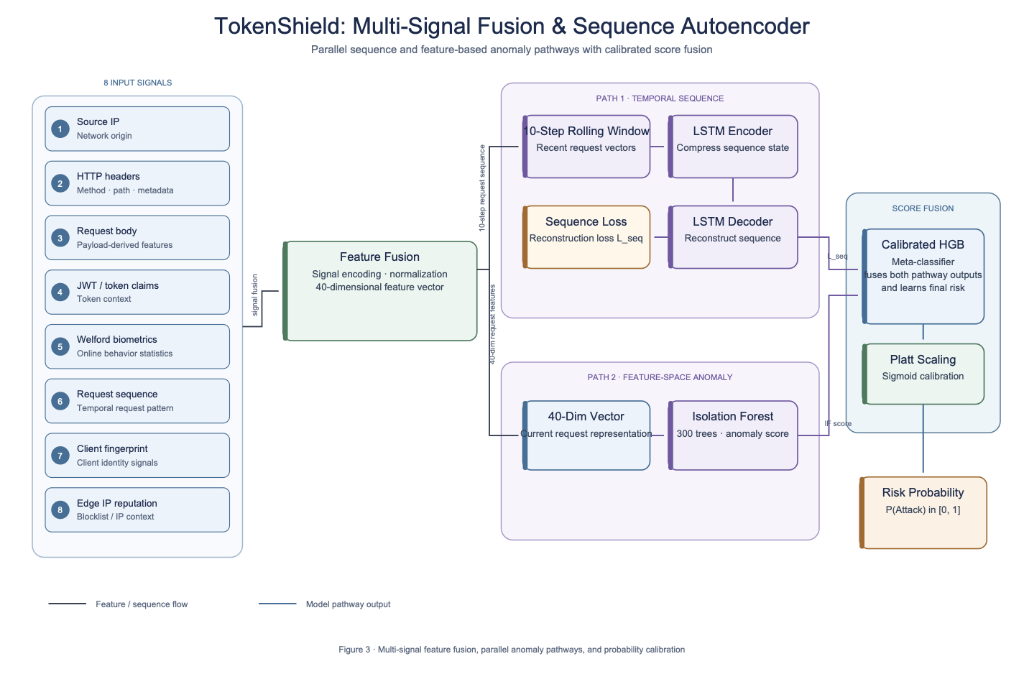
\includegraphics[width=\columnwidth,keepaspectratio]{fig3_multi_signal_fusion.png}
\caption{Multi-signal telemetry fusion: Network indicators, client biometrics, and sequence dynamics ingested into ensemble classifiers.}
\label{fig:fusion}
\end{figure}

\subsection{Calibrated Meta-Classifier Ensemble (Model C)}
The full 40-dimensional feature vector $\mathbf{F} \in \mathbb{R}^{40}$ is ingested by Model C (\texttt{HistGradientBoostingClassifier}), transformed via Platt sigmoid scaling:
\begin{equation}
P(Y = 1 \mid \mathbf{F}) = \frac{1}{1 + \exp\left(A \cdot z(\mathbf{F}) + B\right)}
\label{eq:platt}
\end{equation}
The composite threat score $S \in [0.0, 1.0]$ triggers progressive operational actions:
\begin{equation}
\text{Action}(S) = \begin{cases}
\text{ALLOW}, & S < 0.60 \\
\text{STEP-UP MFA}, & 0.60 \le S < 0.85 \\
\text{AUTONOMOUS BLOCK}, & S \ge 0.85
\end{cases}
\label{eq:action}
\end{equation}

\section{Automated Mitigation Pipeline}

When high-confidence threats cross threshold boundaries ($S \ge 0.85$), TokenShield deploys an 8-stage asynchronous mitigation pipeline:
\begin{itemize}
    \item \textbf{Stage 1: Redis Token Revocation ($\sim$0\,ms):} Token identifier written to Redis blacklist (TTL 24 hours).
    \item \textbf{Stage 2: Edge IP Block ($\sim$0\,ms):} Attacker's originating IP address blocked in volatile block list.
    \item \textbf{Stage 3: Dynamic Nginx Edge Sync ($\le$5\,s):} IP added to Nginx blocklist; background watcher reloads Nginx gracefully.
    \item \textbf{Stage 4: Device Fingerprint Blacklisting ($\sim$0\,ms):} Fingerprint hash banned in Redis for 72\,hr.
    \item \textbf{Stage 5: Account Hard Lockout ($\sim$10\,ms):} User record flagged in relational database, requiring out-of-band identity verification.
    \item \textbf{Stage 6: Subnet /24 Quarantine ($\sim$10\,ms):} Progressive throttle applied to entire subnet when two or more events originate within a 60\,s window.
    \item \textbf{Stage 7: Asynchronous SOC Alert:} Incident payload dispatched via SMTP to the SOC security queue.
    \item \textbf{Stage 8: Live Dashboard SSE Push:} Real-time threat telemetry streamed via Server-Sent Events to the administrator monitoring console.
\end{itemize}

\section{Experimental Evaluation}

\subsection{Empirical Dataset Corpus (958,534 Records)}
TokenShield was evaluated on an empirical corpus of 958,534 real-world records consolidated across 12 processing pipelines and 23 public sub-corpora:
\begin{itemize}
    \item \textbf{Group A (Network \& Web Telemetry --- 584,210 rows):} UNSW-NB15 (175,341 rows)~\cite{ref5}, CIC-IoT 2023 (200,000 rows)~\cite{ref13}, NSL-KDD (125,973 rows), Bot-IoT (73,360 rows), CSIC 2010 HTTP, and RT-IoT 2022.
    \item \textbf{Group B (Behavioral Biometrics --- 214,324 rows):} CMU Keystroke Dynamics Benchmark (80,000 instances)~\cite{ref11}, Balabit Mouse Dynamics Challenge (54,324 rows), and KeyRecs Keystroke Dataset (80,000 rows).
    \item \textbf{Group C (Sequential Workflow Logs --- 160,000 rows):} NASA HTTP access logs (60,000 rows) and Wikipedia Clickstream logs (100,000 transitions).
\end{itemize}
The dataset was partitioned into a 70\% training split (670,972 samples), a 15\% validation split (143,781 samples), and a 15\% held-out test split (143,781 samples).

\begin{table}[!htbp]
\caption{Feature-Level Comparison With Related Works\\{\normalfont($\checkmark$ = Supported, $\times$ = Not Supported, P = Partial)}}
\label{tab:comparison}
\centering
\resizebox{\columnwidth}{!}{%
\renewcommand{\arraystretch}{1.25}
\begin{tabular}{|l|c|c|c|c|c|c|}
\hline
\textbf{System / Model} & \textbf{Multi-Signal} & \textbf{Biometrics} & \textbf{Sequence} & \textbf{Unsupervised} & \textbf{Calibrated} & \textbf{Mitigation} \\ \hline\hline
Liu et al.\ (iForest)~\cite{ref3} & $\times$ & $\times$ & $\times$ & $\checkmark$ & $\times$ & $\times$ \\ \hline
Freeman et al.~\cite{ref6} & P & $\times$ & $\times$ & $\times$ & $\checkmark$ & $\times$ \\ \hline
TypeNet~\cite{ref10} & $\times$ & $\checkmark$ & $\checkmark$ & $\times$ & $\times$ & $\times$ \\ \hline
Traditional WAF & $\times$ & $\times$ & $\times$ & $\times$ & $\times$ & P \\ \hline
\textbf{TokenShield (Ours)} & $\boldsymbol{\checkmark}$ & $\boldsymbol{\checkmark}$ & $\boldsymbol{\checkmark}$ & $\boldsymbol{\checkmark}$ & $\boldsymbol{\checkmark}$ & $\boldsymbol{\checkmark}$ \\ \hline
\end{tabular}%
}
\end{table}

\begin{table}[!htbp]
\caption{Quantitative Evaluation on 143,781 Held-Out Samples}
\label{tab:quant}
\centering
\resizebox{\columnwidth}{!}{%
\renewcommand{\arraystretch}{1.25}
\begin{tabular}{|l|l|c|l|}
\hline
\textbf{Model Component} & \textbf{Evaluation Metric} & \textbf{Benchmark} & \textbf{Target / Industry Benchmark} \\ \hline\hline
\multirow{5}{*}{\textbf{Model A: Isolation Forest}}
& Precision & \textbf{90.22\%} & High Purity Outlier Filter \\ \cline{2-4}
& False Positive Rate (FPR) & \textbf{4.79\%} & Target $\le 5.0\%$ \\ \cline{2-4}
& Recall (Sensitivity) & \textbf{40.56\%} & Baseline Outlier Separation \\ \cline{2-4}
& PR-AUC & \textbf{0.7600} & Stable Separation Baseline \\ \cline{2-4}
& Inference Latency & \textbf{2.47\,ms} & Sub-5\,ms Critical Budget \\ \hline\hline
\multirow{8}{*}{\textbf{Model C: Meta-Classifier}}
& ROC-AUC Score & \textbf{0.8943} & Discriminative Separation \\ \cline{2-4}
& PR-AUC & \textbf{0.8683} & Balanced Precision-Recall Area \\ \cline{2-4}
& Recall ($\tau = 0.50$) & \textbf{96.90\%} & High-Sensitivity Anomaly Catch \\ \cline{2-4}
& Precision ($\tau = 0.50$) & \textbf{72.52\%} & Raw Operating Precision \\ \cline{2-4}
& FPR ($\tau = 0.50$) & \textbf{40.03\%} & First-Pass Alarm Baseline \\ \cline{2-4}
& Precision ($\tau \ge 0.85$) & \textbf{98.18\%} & High-Confidence Enforcement \\ \cline{2-4}
& FPR ($\tau \ge 0.85$) & \textbf{1.05\%} & Ultra-Low False Alarm Rate \\ \cline{2-4}
& Training Time (Apple M2) & \textbf{85.09\,s} & Local Silicon Convergence \\ \hline\hline
\multirow{2}{*}{\textbf{Hardware (Apple M2)}}
& Avg.\ Inference Latency & \textbf{11.25\,ms} & Sub-50\,ms SLA \\ \cline{2-4}
& P95 Latency & \textbf{14.97\,ms} & Deterministic Real-Time Budget \\ \hline
\end{tabular}%
}
\end{table}

\subsection{Confusion Matrix Verification (143,781 Evaluated Instances)}
At the default operating threshold ($\tau = 0.50$), Model C correctly classified 72,670 True Positives (TP) and 41,252 True Negatives (TN), with only 2,328 False Negatives (FN) and 27,531 False Positives (40.03\% FPR, 72.52\% precision). When evaluated at the calibrated autonomous mitigation threshold ($\tau \ge 0.85$), false alarms drop sharply to 1.05\% FPR with 98.18\% precision, confirming that disruptive mitigations are enforced strictly on high-confidence threats.

\subsection{Live Attack Verification Matrix (\texttt{demo\_test.py})}
To validate the system under real-world runtime conditions, TokenShield was tested against 5 live attack vectors:
\begin{itemize}
    \item \textbf{Benign User Navigation:} Valid token, consistent IP $\to$ Allowed ($S = 0.04$, Latency: 7.26\,ms).
    \item \textbf{Session Hijacking via Tor:} Token replayed from Tor exit IP 185.220.101.5 $\to$ Flagged ($S = 0.81$, Latency: 4.94\,ms, Stage 1--2 triggered).
    \item \textbf{Payload Injection:} SQLi string in transaction payload $\to$ Blocked ($S = 0.90$, Latency: 7.86\,ms).
    \item \textbf{Biometric Account Takeover:} Automated bot typing (165 WPM) $\to$ Blocked ($S = 0.90$, Latency: 6.20\,ms).
    \item \textbf{Workflow Bypass:} Direct leap to \texttt{/api/transfer/execute} $\to$ Blocked ($S = 0.90$, Latency: 36.43\,ms).
\end{itemize}

\section{Discussion and Limitations}

\subsection{Privacy-Preserving Architecture}
TokenShield generates only streaming statistical summaries via Welford's algorithm rather than recording raw keystrokes. Neither raw strings nor passwords leave the client runtime memory boundary. Nevertheless, under regulatory regimes such as GDPR, persistent canvas fingerprints and behavioral biometrics may be categorized as pseudonymous personal data, requiring explicit enterprise compliance disclosures.

\subsection{Benchmark Proxy Evaluation and Threat Models}
A fundamental limitation in network intrusion research is the absence of public corpora with authentic session hijacking labels. In our evaluations, proxy data combining network anomalies, biometric impostor dynamics, and sequential workflow jumps was used as an empirical proxy for post-authentication hijacking. In adversarial scenarios where an attacker compromises the victim's host directly and replays tokens from the victim's browser, IP and fingerprint drift signals will not trigger, shifting detection burden onto biometric cadence and sequential navigation. Furthermore, automated /24 subnet quarantine presents collateral denial-of-service risks in environments sharing Carrier-Grade NAT (CGNAT) or institutional proxies.

\section{Conclusion}
In this paper, we described TokenShield, a behavior, multi-signal engine working in real time and which is domain-agnostic with an eight-stage mitigation pipeline for session hijacking detection and instantaneous mitigation. The ability of TokenShield to detect attacks against the same token with a stateless bearer is based exclusively on the evaluation of every authenticated HTTP request as an autonomous trust decision rather than on login-phase-only authentication. Evaluated on a real-world benchmark of 143,781 held-out samples from 23 public sub-corpora, the system demonstrated an ROC-AUC of 0.8943, reaching 96.90\% recall at its triage threshold and achieving 98.18\% precision at 1.05\% false positive rate under its calibrated autonomous mitigation threshold, with an average inference latency of 11.25 ms on commodity Apple M2 hardware.

\begin{thebibliography}{15}

\bibitem{ref1}
M.~Jones, J.~Bradley, and N.~Sakimura, ``JSON Web Token (JWT),'' IETF RFC 7519, May 2015.

\bibitem{ref2}
OWASP Foundation, ``OWASP Top 10:2021 -- Identification and Authentication Failures,'' 2021. [Online]. Available: \url{https://owasp.org/Top10/}

\bibitem{ref3}
F.~T.~Liu, K.~M.~Ting, and Z.-H.~Zhou, ``Isolation Forest,'' in \emph{Proc. IEEE ICDM}, Pisa, Italy, 2008, pp. 413--422.

\bibitem{ref4}
I.~Sharafaldin, A.~H.~Lashkari, and A.~A.~Ghorbani, ``Toward Generating a New Intrusion Detection Dataset,'' in \emph{Proc. ICISSP}, 2018, pp. 108--116.

\bibitem{ref5}
N.~Moustafa and J.~Slay, ``UNSW-NB15: A Comprehensive Data Set for Network Intrusion Detection Systems,'' in \emph{Proc. MilCIS}, Canberra, Australia, 2015, pp. 1--6.

\bibitem{ref6}
D.~Freeman, S.~Jain, M.~D{\"u}rmuth, B.~Biggio, and G.~Giacinto, ``Who Are You? A Statistical Approach to Measuring User Authenticity,'' in \emph{Proc. NDSS}, San Diego, CA, 2016.

\bibitem{ref7}
P.~Eckersley, ``How Unique Is Your Web Browser?,'' in \emph{Proc. PETS}, 2010, pp. 1--18.

\bibitem{ref8}
N.~Nikiforakis et al., ``Cookieless Monster: Exploring the Ecosystem of Web-Based Device Fingerprinting,'' in \emph{Proc. IEEE S\&P}, 2013, pp. 541--555.

\bibitem{ref9}
K.~S.~Killourhy and R.~A.~Maxion, ``Comparing Anomaly-Detection Algorithms for Keystroke Dynamics,'' in \emph{Proc. IEEE/IFIP DSN}, 2009, pp. 125--134.

\bibitem{ref10}
A.~Acien, A.~Morales, J.~V.~Monaco, R.~Vera-Rodriguez, and J.~Fierrez, ``TypeNet: Deep Learning Keystroke Biometrics,'' \emph{IEEE Trans. Biometrics, Behaviour, and Identity Science}, vol. 4, no. 1, pp. 57--70, 2021.

\bibitem{ref11}
K.~S.~Killourhy and R.~A.~Maxion, ``Keystroke Dynamics -- Benchmark Data Set,'' Carnegie Mellon University, 2009. [Online]. Available: \url{https://www.cs.cmu.edu/~keystroke/}

\bibitem{ref12}
R.~Shadman et al., ``Keystroke Dynamics -- Concepts, Techniques, and Applications,'' \emph{ACM Computing Surveys}, vol. 58, no. 3, Article 50, 2025.

\bibitem{ref13}
A.~R.~Punia, S.~S.~Gill, R.~Buyya, et al., ``A Machine Learning-Based Efficient Anomaly Detection Framework for Securing IoT Environments,'' \emph{Internet of Things}, vol. 31, 2025, Art. no. 101573.

\bibitem{ref14}
D.~Fett, B.~Campbell, J.~Bradley, et al., ``OAuth 2.0 Demonstrating Proof-of-Possession at the Application Layer (DPoP),'' IETF RFC 9449, Sep. 2023.

\bibitem{ref15}
OWASP Foundation, ``OWASP API Security Top 10 -- 2023,'' [Online]. Available: \url{https://owasp.org/www-project-api-security/}

\end{thebibliography}

\end{document}
